A study to find the optimal fiber length was carried out. Two different lengths of scintillating fibers, $1~\meter$ and $20~\cm$, and two different tritium source activities, $0.5~\kilo\becquerel/\liter$ and $2.5~\kilo\becquerel/\liter$, were used. Five detectors were simulated for the case of a $20~\cm$ fiber length to have the same active area than for $1~\meter$ length. The advantage of using long fibers is their large active area for the same number of photosensors which would reduce the price of the TRITIUM monitor. However, short scintillating fibers reduce photon absorption, which increases the tritium detection efficiency per unit of active area. 

The Tritium-Aveiro prototype, consisting of $360$ scintillating fibers of $2~\mm$ diameter, was simulated. The number of photons produced in a scintillating fiber per tritium electron for all the electrons that reach the scintillating fibers and for only those that generate photons detected in coincidence by the photosensors are plotted in Figure \ref{fig:PhotonsFibersYesNoPhotosensors}. Tritium events that produce a large number of photons are almost always detected but events that produce few photons are seldom detected, resulting in a peak centred at around $25$ photons.  
\begin{figure}[h]
\centering
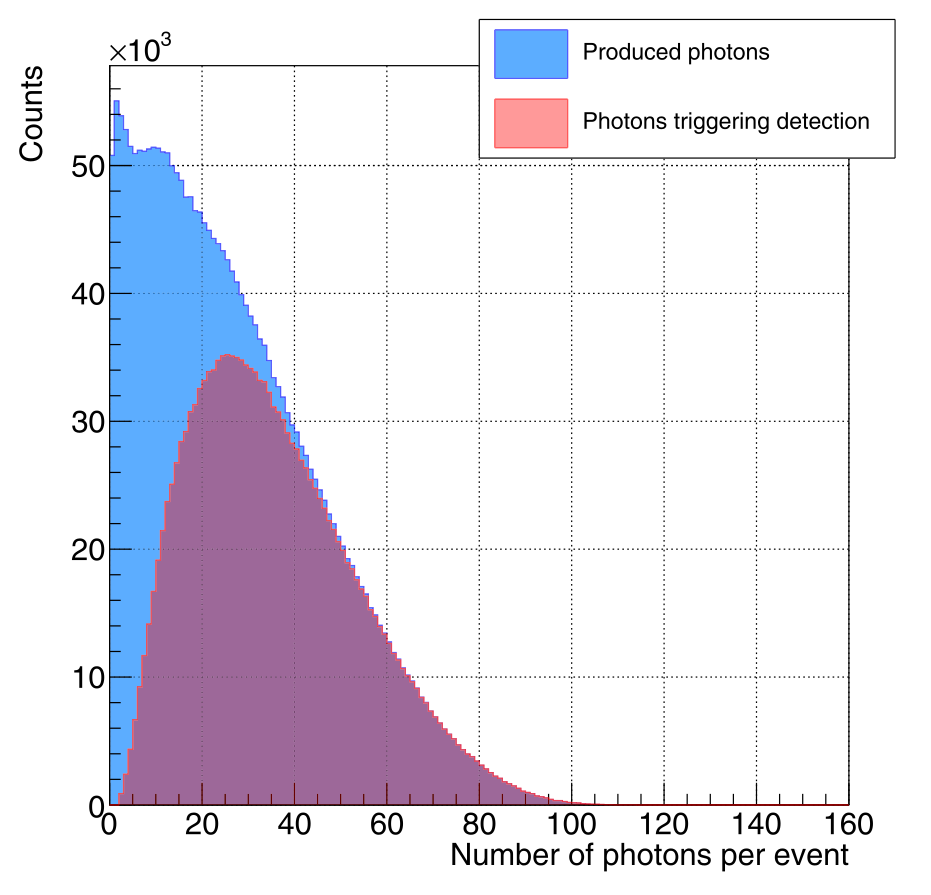
\includegraphics[scale=0.3]{6Simulations/61TRITIUMDesign/613Length/CollectionPhotonsInFibers.png}
\caption{Number of photons produced in a fiber per tritium event for all tritium electrons that reach the fiber (blue histogram) and for only tritium electrons producing photons detected in coincidence by photosensors (red histogram) \cite{SimulationPaperCarlos}.\label{fig:PhotonsFibersYesNoPhotosensors}}
\end{figure}
The number of counts per hour during a week is shown in Figure \ref{fig:CountsOver60minDifferentLength} as a function of time for the tritium activities and fiber lengths studied. A signal 5 times larger is seen for the shorter fiber length and the two activities considered, due mainly to the lower absorption and the refraction loss of photons in shorter fibers. In addition, effects like dirt and mechanical imperfections of fiber surface not simulated increase this photon loss effect.

\begin{figure}[h]
\centering
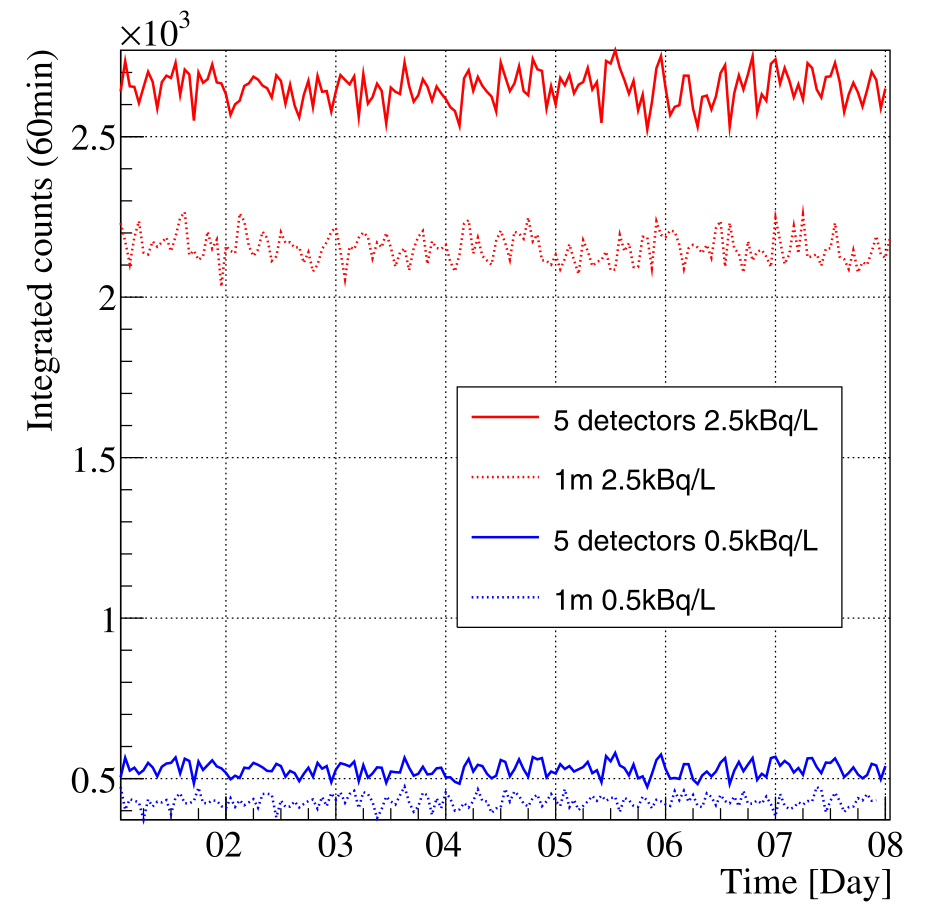
\includegraphics[scale=0.3]{6Simulations/61TRITIUMDesign/613Length/2DifferentLength.png}
\caption{Simulated counting statistics normalized to the active area in $1~\hour$ bins during a week for $1~\meter$ (dashed lines) and $20~\cm$ (solid lines) and $0.5~\kilo\becquerel/\liter$ (blue lines) and $2.5~\kilo\becquerel/\liter$ (red lines) activities \cite{SimulationPaperCarlos}. \label{fig:CountsOver60minDifferentLength}}
\end{figure}

